\section{Case Study: ThingSat}
\label{sec:case-study}

%\subsection{Overview}
% \paragraph*{Mission Goal:} in-orbit observation of glaciers in Europe and in Polynesia.
% \paragraph*{Approach}: rent "rack" space as payload on a CubeSat (SatRevolution).

The Thingsat project~\cite{git:thingsat-repo} aims to benchmark the LoRa links in the context of
space-ground communication for several frequency bands and demonstrate the
effectiveness of that technology inside a LEO (Low Earth Orbit) cubesat.

Thingsat is deployed as a payload hosted on a shared 3U CubeSat: \href{https://space.skyrocket.de/doc_sdat/stork-1.htm}{STORK-1} from the polish start-up \href{https://www.satrevolution.com/}{SatRevolution}. The cubesat was launched on January 13th, 2022,currently in orbit at an altitude of 525 km (see its 
\href{https://www.n2yo.com/database/?q=STORK-1\#results}{Two-Line Elements}).

The Thingsat payload now in orbit is used for Ocean level monitoring.
However, its design can be adequate for a wider variety of use cases, in Earth science academic research (e.g. melting of glaciers, pirate fishing...) and in the industry for companies using geographically dispersed devices (e.g. monitoring of tank ships...). 

\iffalse
Thus we designed a space electronic board with two LoRa transceivers and a patch
antenna operating in 868MHz and 2.4GHz. 
This payload is hosted in a shared 3U
CubeSat - \href{https://space.skyrocket.de/doc_sdat/stork-1.htm}{STORK-1} from
the polish start-up \href{https://www.satrevolution.com/}{SatRevolution}. The
cubesat was launched on January 13th, 2022 on a near-polar orbit at an
altitude of 525 km (See
\href{https://www.n2yo.com/database/?q=STORK-1\#results}{Two-Line Elements}).
\fi


\begin{figure}[t]
    \centering
    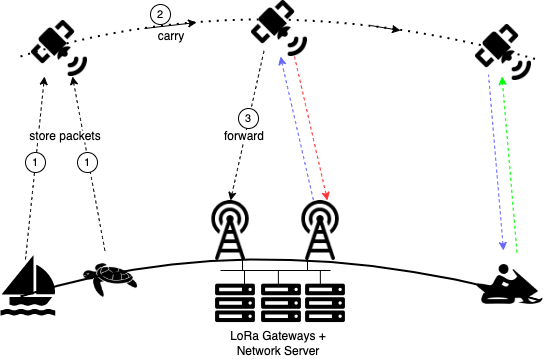
\includegraphics[width=0.5\textwidth]{Figures/thingsat-dtn.png}
    \caption{ThingSat in-orbit communication patterns.}
    \label{fig:thingsat-comm}
\end{figure}


% \paragraph*{High-level overview of Segments}

\subsection{Distributed System Architecture}

The figure \ref{fig:thingsat-archi} describes the Thingsat deployment components, which gives an
overview of a typical cubesat ecosystem hosting a payload, whereby the interaction with this payload traverses unstrusted elements.

\begin{figure}[ht]
    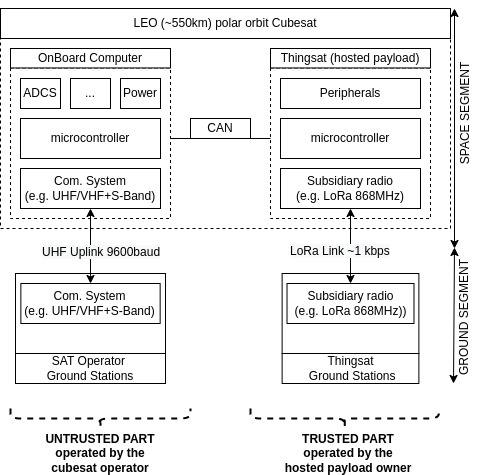
\includegraphics[width=0.5\textwidth]{Figures/globecom-thingsat-mods.jpg}
    \caption{ThingSat hosted payload: deployed components and architecture.}
    \label{fig:thingsat-archi}
\end{figure}

% \paragraph*{Space Segment Description}
The \textit{Space Segment}  comprises especially the OBC and payloads sharing resources of the cubesat, interconnected via a CAN bus.
The OBC
consists of a microcontroller with all its subsystems to operate the cubesat :
the Attitude Determination and Control System, the communication subsystems
(UHF/VHF/S-band for uplink/downlink + antennas), the power subsystem (Battery
Management, Energy Harvesting with Solar Panels, Auxiliary Power Supply). The
payload designed for the Thingsat project embeds both a
\href{https://www.semtech.com/products/wireless-rf/lora-gateways/sx1302}{Semtech
SX1302 transceiver} for communications on the 863-870 MHz band and a
\href{https://www.semtech.com/products/wireless-rf/24-ghz-transceivers/sx1280}{Semtech
SX1280 transceiver} for communications on the 2400-2500 MHz band. Furthermore a dual-band patch antenna (868MHz, 2.4GHz) was designed. The firmware running on the STM32 microcontroller driving LoRa communications is based on \href{https://github.com/RIOT-OS/RIOT}{RIOT
OS}.

% \paragraph*{Ground Segment Description}
% \paragraph*{Control Segment} % Francisco: not sure if its the right name

For the \textit{Ground Segment}, the cubesat operator relies on 
i) Ground
Stations\footnote{not necessarily owned by the cubesat operator} to communicate
with the OBC and 
ii) a Command \& Control Center to operate the cubesat
(telecommand/telemetry) and to provide a means for payload maintainers to
interact with the hosted payload.

% \paragraph*{OBC \& Payload Communication Bus}

% \paragraph*{Payload Description}: tenant status, energy budget, on time etc.
% - OBC -> SatRev controlled
% - Payload -> Full Control

\subsection{Communication Characteristics Overview}
\label{sec:thingsat-comm-characteristics}
% \paragraph*{link-budget Mission Control}: delivering and communicating mission
% files, delivering software updates, latency, etc.

The Thingsat payload communicates either directly via LoRa, or indirectly via the UHF link provided by the cubesat's OBC.

\paragraph*{Direct communication patterns}
LoRa communication patterns are illustrated in figure \ref{fig:thingsat-comm}.
Thingsat can communicate directly with its LoRa interface, with LoRa network elements on the ground.

As depicted, the Thingsat payload may act in turns as either 
(i) a Sat-IoT end-device (ED) that will send Lora frames to terrestrial LoRaWAN gateways or Thingsat ground stations (GS), or 
(ii) an in-orbit LoRa sniffer, or 
(iii) a store-carry-and-forward LoRa gateway.

Patterns (i) and (ii) allow to benchmark simple ground-space LoRa links by
making statistics over multiple sent/received frames. Pattern (iii) is a more
complex scenario: the satellite stores packets received from GS/ED and deliver
them once GS/ED destinations are inside the footprint of the satellite.

\paragraph*{Indirect communication characteristics}
Communication with cubesats are typically done on amateur frequency
bands (UHF/VHF) with typically low data rates ranging from 9.6kbps to
100kbps. 
Generally, over a given ground station, a polar LEO satellites carries out an average of 2-4 passes per day. The duration of the communication window is approximately of 5 to 10
minutes. 

In the particular case of Thingsat, we have only 2 ground stations to interact with the cubesat and a 10-kbps
link, the data that can be exchanged during a day is roughly 1500KB (= 2 GS x 2
passes/day x 5-min pass x 10kbps). This amount should be shared between OBC
(for telecommand/telemetry/update) and hosted payload communications. To give an
idea, the total communication budget available for Thingsat via UHF/VHF is thus 300KB per day. \todoOA{See with SR for details}


% \paragraph*{link-budget Mission}: communication between OBC and Payload, payload
% active time for communication with ground segments.
\iffalse
Regarding the communication with the OBC, an API is provided to the hosted
payload to read/write data with the data handling module of the cubesat as well
as interacting with its subsystems. Indeed, to carry out a provisioned mission,
the payload needs information from the OBC : awaiting uploaded
instructions/files, GPS, time, ADCS, time before shutdown, ...
\fi

Last but not least, the Thingsat payload is not powered on at all times.
Typically on such a cubesat, the power available is only
enough for one active payload at a time. 
%The mission of the STORK constellation is earth observation. So each STORK cubesat is equipped with an imager~\cite{wiki:SatRevolution} which has its own missions.
The OBC is in charge of turning on the relevant payload according to a schedule
uploaded from the ground station. 

To give an idea, when active and using the 863-870 MHz band, the
Thingsat payload consumes at 3.3V : 
(i) 90 mA in standby, 
(ii) 110 mA during a frame reception (RX) and 
(iii) 300 mA during a frame transmission (TX) at 27 dBm.

\subsection{Data and Software Updates Requirements}

% \paragraph*{Why?}: timeline for deployment, CoVID context, etc. making it impossible
% to deliver a fully functional device in time. Need to update the firmware remotely
% and in orbit.

The data exchanged by the Payload Maintainer with the Thingsat payload comprises 
\begin{itemize}
    \item the delivery of mission files running above the same firmware and the
    recovery of experiment results
    \item firmware updates
    \item diagnostic files to help the debug of failed missions/updates
\end{itemize} 

\todoOA{be more specific on those files (discuss with Didier + give typical size of files}

% The ability to reprogram the cubesat in orbit is essential for academic projects like Thingsat. First the design, development and deployment life-cycles of cubesat projects are quite short and the financial budget in academic projects is limited. Secondly the academic development team (students, professors, engineers) are at best experts in their respective domain but not necessarily familiar with space systems. Those constraints makes it impossible to deliver a fully functional device in time. The COVID context aggravated the situation with forced remote working, electronic component shortages and delayed shippings. 

% \paragraph*{What needs updates}: Missions ? 

Concerning software update in particular, while in orbit, Thingsat must be able to
\begin{itemize}
    \item update/add functionalities such as radio drivers  etc.
    \item update mission scenarios
    \item update configuration files
    \item update firmware to fix bugs
\end{itemize} 
%sIn-orbit software updates must allow for updating radio drivers, the evolution of missions scenarios or configurations file format, bug resolutions ...
% Fortunately the use of RIOT-OS greatly facilitates the process to update softwares \textcolor{red}{but still needed adaption to our context}.

% \paragraph*{Communication Chain}: how are new firmware, payloads delivered,
% who has access, etc..
At last, the update of softwares like the Firmware (FW) for instance goes
through the following steps : i) the FW is uploaded to the cubesat by the
payload maintainer (PO) through one of the cubesat operator (CO) ground
stations, ii) once the payload is turned on and reset, it asks the OBC for any
awaiting files/instructions to execute, iii) the OBC uploads the FW chunk by
chunk to the payload and iv) the FW update is triggered by the payload. This
process provided by the CO going through the untrusted parts identified in
figure \ref{fig:thingsat-archi} led us to provide the secured process detailed in the
next section.
